\documentclass[a4paper]{article}
\usepackage[14pt]{extsizes}
\usepackage{amssymb}  %  Математические символы
\usepackage{amsmath}  %  Математический пакет
\usepackage{amsthm}  %  Пакет для использования теорем
\usepackage{caption}  %  Пакет для использования подписей
\usepackage{misccorr}  %  Пакет с большинством настроек русских типографических правил - точки после цифр в оглавлении, etc.
\usepackage[noadjust]{cite}
\usepackage{cmap} % Для возможности нормального поиска в тексте и копирования!
\usepackage[utf8]{inputenc}  %  Кодировка исходного файла, который я тут вижу
\usepackage[T2A]{fontenc}  %  Набор символов на выходе, T2A включает в себя кириллицу
\usepackage[german, english, russian]{babel}
\usepackage{graphics}
\usepackage{graphicx}
\usepackage{indentfirst}  %  Либо подключать этот пакет, либо писать каждый раз \indentfirst в начале каждой главы (на Западе не ставят первую красную строку)
\usepackage{verbatim}  %  Окружение для вставки raw-кода
\usepackage{makeidx}
\usepackage{geometry}  %  Настройка геометрии вёрстки -- например, полей
\usepackage{hyperref}
\usepackage{fancyvrb}
\usepackage{color} %% это для отображения цвета в коде
\usepackage{listings} %% собственно, это и есть пакет listings
\usepackage{wrapfig}
\usepackage{setspace}
\usepackage{mathabx}
\usepackage{mathtools}

\DeclareCaptionFont{white}{\color{white}} %% это сделает текст заголовка белым
\DeclareCaptionFormat{listing}{\colorbox{gray}{\parbox{\textwidth}{#1#2#3}}}
\captionsetup[lstlisting]{format=listing,labelfont=white,textfont=white}
\DeclareGraphicsExtensions{.pdf,.png,.jpg}
\newcommand{\suml}{\sum\limits}  %  Свои, русские суммы
\geometry{pdftex, left = 2cm, right = 2cm, top = 2.5cm, bottom = 2.5cm}
\righthyphenmin = 2

\begin{document}
	\begin{titlepage}
		\centering
		\begin{wrapfigure}[7]{l}{0.14\linewidth}
			\vspace{5mm}
			\hspace{-5.8mm}
			
\includegraphics[width=0.93\linewidth]{gerb}
		\end{wrapfigure}
		{\singlespacing \footnotesize \bfseries Министерство науки и высшего образования Российской Федерации\\Федеральное государственное бюджетное образовательное учреждение\\высшего образования\\<<Московский государственный технический университет\\имени Н.~Э.~Баумана\\ (национальный исследовательский университет)>>\\(МГТУ им. Н.~Э.~Баумана)\\}
		
		\textbf {\bf \underline{\hspace{\linewidth}}}
		\doublespacing \small \raggedright ФАКУЛЬТЕТ \hspace{25mm} \underline { «Информатика и системы управления»}\\
		КАФЕДРА \hspace{5mm} \underline {«Программное обеспечение ЭВМ и информационные технологии»}\\
		
		\vspace{30mm}
		\begin{center}
		\textbf{Отчёт по лабораторной работе №2}\\
		{\bf	По дисциплине: <<Анализ алгоритмов>>}\\
		{\bf Тема:} \underline {<<Алгоритмы умножения матриц>>}\\
		\end{center}
		%\vspace{60mm}
		\begin{flushleft}
			{\bf Студент}  \underline{Мередова Айджахан}\underline {\hspace{7cm}}
			\newline
			{\bf Группа} \underline{ИУ7-56Б}\underline {\hspace{10cm}}
		
			{\bf Преподаватели} \underline {Волкова Л.Л., Строганов Ю.В.}
		\end{flushleft}
		\vfill
		
		\centering Москва - 2020 г.\\
	\end{titlepage}
	\lstset{ %
		language=Python,                 % выбор языка для подсветки 
		basicstyle=\small\sffamily, % размер и начертание шрифта для подсветки кода
		%numbers=left,               % где поставить нумерацию строк (слева\справа)
		numberstyle=\tiny,           % размер шрифта для номеров строк
		stepnumber=1,                   % размер шага между двумя номерами строк
		numbersep=5pt,                % как далеко отстоят номера строк от подсвечиваемого кода
		backgroundcolor=\color{white}, % цвет фона подсветки - используем \usepackage{color}
		showspaces=false,            % показывать или нет пробелы специальными отступами
		showstringspaces=false,      % показывать или нет пробелы в строках
		showtabs=false,             % показывать или нет табуляцию в строках
		frame=single,              % рисовать рамку вокруг кода
		tabsize=2,                 % размер табуляции по умолчанию равен 2 пробелам
		captionpos=t,              % позиция заголовка вверху [t] или внизу [b] 
		breaklines=true,           % автоматически переносить строки (да\нет)
		breakatwhitespace=false, % переносить строки только если есть пробел
		escapeinside={\%*}{*)}   % если нужно добавить комментарии в коде
	}
	
	\section*{Введение}
	Матрица - математический объект, эквивалентный двумерному массиву. Числа располагаются в матрице по строкам и столбцам.Две матрицы одинакового размера можно поэлементно сложить или вычесть друг их друга. Если число столбцов в первой матрице совпадает с числом строк во второй, то эти две матрицы можно перемножить. У произведения будет столько же строк, сколько в первой матрице, и столько же столбцов, сколько во второй. Умножение матриц некоммутативно: оба произведения AB и BA двух квадратных матриц одинакового размера можно вычислить, однако результаты, вообще говоря, будут отличаться друг от друга.  
	Умножение матрицы А  размера $m \times n$ и матрицы В  размера $n \times l$ приводит к получению матрицы С размера $m \times l$, каждый элемент которой определяется в соответствии с выражением:
 	\begin{equation}
 		C_{ij} = \suml_{p=1}^{m} a_{ip} * b_{pj}
 	\end{equation}
 	
	\clearpage
	\section {Аналитическая часть}
	\subsection {Постановка задачи}
	Цель данной лабораторной работы: Провести сравнительный анализ алгоритмов умножения матриц и получить навык оптимизации алгоритмов.
	Задачи данной лабораторной работы:
	\begin{enumerate}
		\item Дать математическое описание (формуты рассчётов для алгоритмов);
		\item Реализовать старндартный алгоритм умножения матриц и алгоритм Винограда;
		\item Разработать оптимизированный алгоритм Винограда;
		\item Дать теоретическую оценку трудоёмкости трёх алгоритмов;
		\item Провести замеры процессорного времени работы реализаций алгоритмов;
	\end{enumerate}
	
	\subsection{Описание алгоритма}
	\subsubsection{Последовательный алгоритм умножения матриц}
	Последовательный алгоритм умножения матриц представляется тремя вложенными циклами. 
	\begin{lstlisting}[caption = Последовательный алгоритм умножения матриц]
		MatrixA[n][n]
		MatrixB[n][n]
		MatrixC[n][n]
		for i in range n:
			for j in range n:	
				MatrixC[i][j] = 0
				for k in range n:
					MatrixC[i][j] += MatrixA[i][k] * Matrix[k][j]
		
	\end{lstlisting}
	Этот алгоритм является итеративным и ориентирован на последовательное вычисление строк матрицы С.
	Поскольку каждый элемент результирующей матрицы есть скалярное произведение строки и столбца исходных матриц, то для вычисления всех элементов матрицы  С  размером $n \times n$ необходимо выполнить $n^2x(2n - 1)$ скалярных операций и затратить время
	\begin{equation}
		T_1 = n^2 * (2n-1) * \tau  ,
		\label{time_1}
	\end{equation}

	где $\tau$ есть время выполнения одной элементарной скалярной операции.
	
	\subsubsection{Алгоритм Винограда умножения матриц}
	 Если посмотреть на результат умножения двух матриц, то видно, что каждый элемент в нем представляет собой скалярное произведение соответствующих строки и столбца исходных матриц.
	 Такое умножение допускает предварительную обработку, позволяющую часть работы выполнить заранее.
	 Рассмотрим два вектора $V = (v1, v2, v3, v4)$ и $W = (w1, w2, w3, w4)$. Их скалярное произведение равно:
	 
	 \begin{equation}
	 	V \times W = v1w1 + v2w2 + v3w3 + v4w4.
	 \label{formula_2}
	 \end{equation}
	 
	 Это равенство можно переписать в виде:
	 
	 \begin{equation}
	 	V \times W = (v1 + w2)(v2 + w1) + (v3 + w4)(v4 + w3) - v1v2 - v3v4 - w1w2 - w3w4.
	 \label{formula_3}
	 \end{equation}
 	Кажется, что выражение ~(\ref{formula_3}) задает больше работы, чем ~(\ref{formula_2}): вместо четырех умножений мы насчитываем их шесть, а вместо трех сложений - десять. Менее очевидно, что выражение в правой части последнего равенства допускает предварительную обработку: его части можно вычислить заранее и запомнить для каждой строки первой матрицы и для каждого столбца второй. На практике это означает, что над предварительно обработанными элементами нам придется выполнять лишь первые два умножения и последующие пять сложений, а также дополнительно два сложения.
 	
 	\subsubsection{Вывод}
 	Были рассмотрены алгоритмы последовательного умножения матриц и алгоритм Винограда. Их разница заключается в предварительной обработке скалярного произведения соответствующих строк и столбцов исходных матриц, а также уменьшение количества операций умножения.
 	\subsection{Вычисление сложности алгоритма}
 	Расммотрим сложности операций.
 	\textbf{Операции со сложностью "1":}
 	\begin{enumerate}
 		\item Присваивание <<=>>
 		\item Сложение <<+>>
 		\item Вычитание <<->>
 		\item Унарный плюс <<+>>
 		\item Унарный минус <<->>
 		\item Умножение <<*>>
 		\item Деление <</>>
 		\item Взятие остатка от деления <<\%>>
 		\item Инкремент (префиксный и постфиксный) <<++>>
 		\item Декремент (префиксный и постфиксный) <<- ->>
 		\item Индексация (обращение к элементу массива) <<[]>>
 		\item Присваивание со сложением <<+=>>
 		\item Равенство <<==>>
 		\item Неравенство <<!=>>
 		\item Больше << > >>  
 		\item Меньше << < >>
 		\item Больше или равно << >= >>
 		\item Меньше или равно << <= >>
 		\item Логическое отрицание << ! >>
 		\item Логическое умножение << \&\& >>
 		\item Логическое сложение <<||>>
 		\item Побитовая инверсия << $\sim$ >>  
 		\item Побитовое И <<\&>>
 		\item Побитовое ИЛИ << | >>
 		\item Присваивание со сложением << += >>
 		\item Присваивание с вычитанием << -= >>
		\item Присваивание с умножением << *= >>
		\item Присваивание с делением << /= >>
		\item Присваивание  со взятием остатка от деления << \% = >>
 	\end{enumerate}
 \textbf{Условный оператор:}\\
		if(условие)\\
		\{\\
				// тело условия А \\
		\}\\
		else\\
		\{\\
		// тело условия В\\
		\}\\
	
 	Пусть стоимость перехода к одной из ветвей решения равна 0, тогда трудоёмкость if при $f_(min) = min (f_a, f_b), f_(max) = max(f_a, f_b)$, получим
 	\begin{equation}
 		f_(if) = f + \begin{cases}
 			D(S_1[1..i], S_2[1..j-1]) + 1\\
 			D(S_1[1..i-1], S_2[1..j]) + 1\\
 			\end{cases}
 		\label{formula_4}
 	\end{equation}	
 \textbf{Цикл со счётчиком:}\\
 for (int i =0 ; i < n ; i++)\\
 \{\\
 	//тело цикла\\
 \}\\
 
 Начальная инициализация  int i = 0 выполняется всего один раз - 1 операция. Условие $i < n$ проверяется перед каждой итерацией и при входе в цикл - n + 1 операций. Тело цикла выполняется $n$ раз - $ n * f$. Изменение счётчика $i++$ выполняется на каждой итерации, но перед проверкой условия - $n$ операций. Итого сложность цикла со счётчиком:$2+ n * (2+f)$, где $f$ - сложность тела цикла.
 
 
 \section {Конструкторская часть.}
 \subsection{Схемы алгоритмов.} 
 На рисунках ~\ref{image3} - ~\ref{image6} представлены схемы алгоритмов умножения матриц: стандартного, Винограда и оптимизированного алгоритма Винограда.
 
 \begin{figure}[h]
 	\center{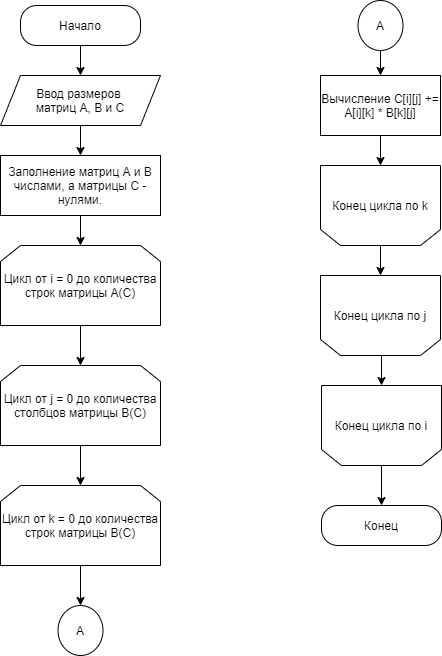
\includegraphics[width=0.8\linewidth, height = 0.8\textheight]{matrix}}
 	\caption{Схема стандартного алгоритма умножения матриц \centering}
 	\label{image3}
 \end{figure}

\begin{figure}[h]
	\center{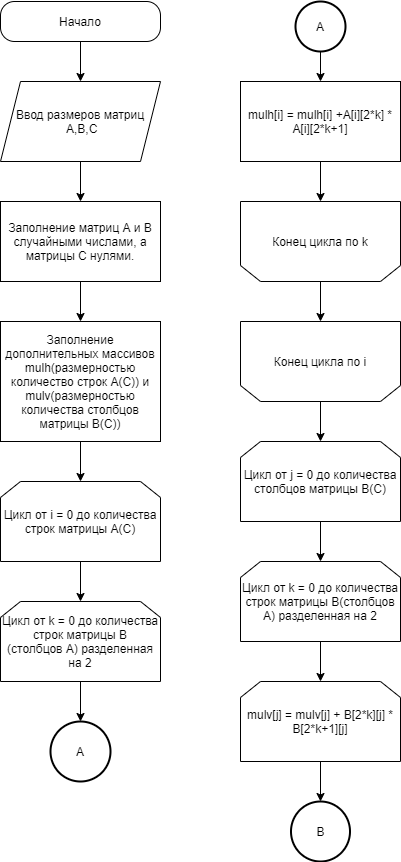
\includegraphics[width=0.8\linewidth, height = 0.8\textheight]{vinograd1}}
	\caption{Схема алгоритма Винограда умножения матриц(1)\centering}
	\label{image4}
\end{figure}

\begin{figure}[h]
	\center{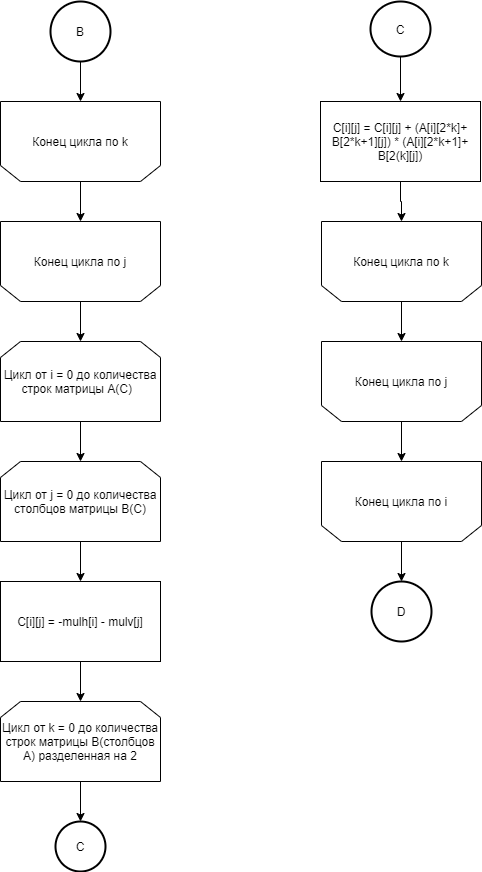
\includegraphics[width=0.8\linewidth, height = 0.8\textheight]{vinograd2}}
	\caption{Схема алгоритма Винограда умножения матриц(2).\centering}
	\label{image5}
\end{figure}

\begin{figure}[h]
	\center{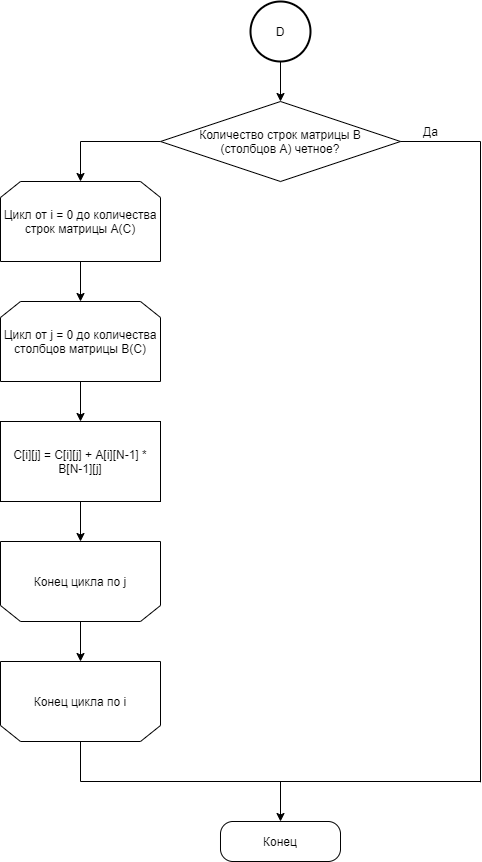
\includegraphics[width=0.8\linewidth, height = 0.8\textheight]{vinograd3}}
	\caption{Схема алгоритма Винограда умножения матриц(3)\centering}
	\label{image6}
\end{figure}
\clearpage
 \section{Технологическая часть}
 \subsection{Выбор языка программирования}
 Python\cite{what_is_python} — это высокоуровневый язык программирования, который используется в различных сферах IT, таких как машинное обучение, разработка приложений, web, парсинг и другие.
 С ним легко работать, что сокращает время разработки. Написанный в удобочитаемом формате, Python делает процесс разработки программного обеспечения быстрым, удобным и максимально упрощенным.
 По сравнению с другими языками, Python в 5-10 раз быстрее по времени разработки, однако медленный при выполнении программ. Он обеспечивает расширенные возможности управления процессами и объектно-ориентированный дизайн, помогая как в скорости, так и в производительности.
 \clearpage
 
 \subsection{Методы замера времени в программе}
 \subsubsection{Время}
 Сушествует несколько способов измерения процессорного времени исполнения программы. 
 Помимо стандратного модуля $time$ есть библиотека $timeit$ \cite{timeit}. Этот модуль предоставляет простой способ найти время выполнения маленьких битов кода Python.
 $timeit$ запускает фрагмент кода миллионы раз(значение по умолчанию - 1000000), так что получаем наиболее статистически значимое измерение времени выполнения кода.
 \subsubsection{Улучшение точности замеров времени} Чтобы получить более точные результаты, каждый тест запускается несколько раз, все полученные значения времени(в тиках) суммируются и делятся на количество запусков кода. Таким образом, получаем среднее время выполнения кода.
 \clearpage
 
 \section{Экспериментальная часть}
 \subsection{Листинг кода}
 В листингах 3 -  представлена реализация стандартного алгоритма умножения матриц, алгоритма Винограда и оптимизированного алгоритма Винограда.
 
 \begin{lstlisting}[label = standart, caption = Стандартный алгоритм умножения матриц]
 	def standart(a, b, c, n, m, q):
 		for i in range (n):
 			for j in range (q):
 				for k in range (m):
 					c[i][j] = c[i][j] + a[i][k] * b[k][j]
 \end{lstlisting}

  \begin{lstlisting}[label = vinograd, caption = Алгоритм Винограда умножения матриц]
  	def vinograd(a, b, c, n, m, q):
	  	mulh = [0 for i in range(n)]
	  	mulv = [0 for i in range(q)]
	  	
	  	for j in range(q):
	  		for k in range(m // 2):
	  			mulv[j] = mulv[j] + (b[2*k][j] * b[2*k+1][j])
	  	
	  	
	  	for i in range(n):
	  		for k in range(m // 2):
	  			mulh[i] = mulh[i] + (a[i][2*k] * a[i][2*k+1])
	  	
	  	for i in range(m):
	  		for j in range(q):
	  			c[i][j] = - mulh[i] - mulv[j]
	  			for k in range(m // 2):
	  				c[i][j] = c[i][j] + (a[i][2*k] + b[2*k+1][j]) * (a[i][2*k+1] + b[2*k][j])
	  				
	  	if m % 2 != 0:
	  		for i in range(n):
	  			for j in range(q):
	  				c[i][j] = c[i][j] + a[i][m-1] * b[m-1][j]
\end{lstlisting}

\begin{lstlisting}[label = optimize_vinograd, caption = Оптимизированный алгоритм Винограда умножения матриц]
	def isOdd(a, b, m, i, j):
		if m % 2 == 0:
			return 0
		return a[i][m-1] * b[m-1][j]
		
	def optimize_vinograd(a, b, c, n, m, q):
		mulh = [0 for i in range(n)]
		mulv = [0 for i in range(q)]
		
		d = m // 2     
		for j in range(q):
			for k in range(d):
				mulv[j] += (b[2*k][j] * b[2*k+1][j])
		
		
		for i in range(n):
			for k in range(d):
				mulh[i] += (a[i][2*k] * a[i][2*k+1])
		
		
		temp = 0
		for i in range(n):
			for j in range(q):
				temp = isOdd(a, b, m, i, j)
				temp -= mulh[i] + mulv[j]
				for k in range(0,d, 2):
					temp += (a[i][2*k] + b[2*k+1][j]) * (a[i][2*k+1] + b[2*k][j])
				c[i][j] = temp
		
\end{lstlisting}
\clearpage

\subsection{Примеры работы}
На таблице 1 приведены примеры работы алгоритмов умножения матриц.
\begin{table}[h]
	\begin{tabular}{lllll}
		\cline{1-4}
		\multicolumn{1}{|l|}{\begin{tabular}[c]{@{}l@{}}А:\\ |-20   -7| \\ |-19 -11|\\  B: \\ |-2   -7 |\\ | 6   -6 |\end{tabular}}                                 & \multicolumn{1}{l|}{\begin{tabular}[c]{@{}l@{}}C: \\ |-2    182|\\ |-28  199|\end{tabular}}                                                                      & \multicolumn{1}{l|}{\begin{tabular}[c]{@{}l@{}}C: \\ |-2   182 |\\ |-28 199 |\end{tabular}}                                                                           & \multicolumn{1}{l|}{\begin{tabular}[c]{@{}l@{}}C: \\ |-2   182|\\  |-28 199|\end{tabular}}                                                                             &  \\ \cline{1-4}
		\multicolumn{1}{|l|}{\begin{tabular}[c]{@{}l@{}}A: \\ | -6  -6|\\ |18  14|\\ |5      4|\\ B: \\ |-16|\\ |-14|\end{tabular}}                          & \multicolumn{1}{l|}{\begin{tabular}[c]{@{}l@{}}C: \\ |180 |\\ \\ |-484| \\ |-136|\end{tabular}}                                                                   & \multicolumn{1}{l|}{\begin{tabular}[c]{@{}l@{}}C: \\ | 180  |\\  |-484 |\\  |-136 |\end{tabular}}                                                                    & \multicolumn{1}{l|}{\begin{tabular}[c]{@{}l@{}}C: \\ | 180  |\\ |-484 |\\  |-136 |\end{tabular}}                                                                    &  \\ \cline{1-4}
		\multicolumn{1}{|l|}{\begin{tabular}[c]{@{}l@{}}A: \\ |-8     3    18| \\  |-13  18    0 | \\ B: \\ |13     3|\\  |-15  17| \\  |1     14|\end{tabular}} & \multicolumn{1}{l|}{\begin{tabular}[c]{@{}l@{}}C: \\ |-131 279|\\  |-439 267|\end{tabular}}                                                                       & \multicolumn{1}{l|}{\begin{tabular}[c]{@{}l@{}}C: \\ |-131 279| \\ |-439 267|\end{tabular}}                                                                           & \multicolumn{1}{l|}{\begin{tabular}[c]{@{}l@{}}C: \\ |-131 279| \\ |-439 267|\end{tabular}}                                                                           &  \\ \cline{1-4}
		\multicolumn{1}{|l|}{\begin{tabular}[c]{@{}l@{}}A:\\ |  9  |\\ |-16 |\\ | -3  |\\ |  11 |\\  B:\\ | 1 16 15 |\end{tabular}}                              & \multicolumn{1}{l|}{\begin{tabular}[c]{@{}l@{}}C: \\ | 9      144     135 | \\  |-16  -256  -240 |\\  |-3     -48    -45  |\\  |11    176    165 |\end{tabular}} & \multicolumn{1}{l|}{\begin{tabular}[c]{@{}l@{}}C: \\ |9       144     135| \\ |-16   -256   -240|\\  |-3      -48     -45 |\\  |11     176     165|\end{tabular}} & \multicolumn{1}{l|}{\begin{tabular}[c]{@{}l@{}}C: \\ |9       144     135| \\ |-16   -256   -240|\\  |-3       -48    -45 |\\  |11      176    165|\end{tabular}} &  \\ \cline{1-4}

	\end{tabular}
\end{table}
\clearpage
\subsection{Оценка трудоёмкости}
\begin{enumerate}
	\item Стандартный алгоритм:
	$f_{std} = 2 + N (2 + 2 + Q(2 + 2 +M(2+1+8+1+1))) = 13 NMQ + 4NQ + 4N + 2 \approx 13NMQ \label{formula_standart}$
	
	\item Алгоритм Винограда:\\
	\begin{equation}
		f_{v1+} = 2 + N(2 + 2 + 3 + \dfrac{N}{2}(3 + 1 + 6 + 2 + 3 + )) = \dfrac{15}{2}MN + 7N + 2 \approx \dfrac{15}{2}MN  \label {vinograd1}
	\end{equation}
	
	\begin{equation}
		f_{v1} = 2 + N(2+2+2+\dfrac{N}{2}(2+5+1+1+1)) = 10NM + 6N + 2  \approx  \dfrac{10}{2} NM = 5NM \label{vinograd2}
	\end{equation}
	
	\begin{equation}
	f_{v2} = 2 + Q(2+2+3+ \dfrac{N}{2}(3+6+1+2+3)) = \dfrac{15}{2} QM + 7Q + 2 \approx \dfrac{15}{2}QM  \label{vinograd3}
	\end{equation}
	
	\begin{equation}
	f_{v2+} = 2+Q(2+2+\dfrac{Q}{2}(2+5+1+1+1)) = 10QM + 6Q+2 \approx \dfrac{10}{2}QM = 5QM \label {vinograd4}
	\end{equation}
	
	\begin{equation}
	f_{v3} = 2+N(2+2+Q(2+7+3+\dfrac{N}{2}(3+12+1+5+5)))  = \dfrac{26}{2}NMQ + 12NQ + 4N+2  \approx \dfrac{26}{2} NMQ = 13NMQ \label{vinograd5}
	\end{equation}

	Лучший случай 0,\\
	Худший случай $f_{v4}$
	\begin{equation}
	f_{v4} = 3+ N(2+2+Q(2+13)) = 15QN + 4N + 3 \approx 15QN \label{vinograd 6}
	\end{equation}
	
	В формуле ~(\ref{vinograd 7}) внутри цикла внесен $f_{v4}$ из формулы ~(\ref{vinograd 6}). Поэтому появляются лучший и худший случаи.
	
	\begin{equation}
		f{v3+} = 3+2+N(2+2+Q(2+6+\left[
		\begin{matrix}
			$л.с$., 0\\
			$х.с$., 6+2+1+1\\
		\end{matrix}
	\right] + 2 + \dfrac{N}{2}(2+10+1+2+2+1)))	
	\label{vinograd 7}	
	\end{equation}

	В худшем случае = 9NMQ + 10NQ + 4N + 5\\
	В лучшем случае $\approx$   8NMQ
	
	\begin{equation}
		f_{v} = f_{v1} + f_{v2} + f_{v3} + f_{v4} = \dfrac{15}{2}NM + \dfrac{15}{2} QM + \dfrac{26}{2}NMQ + 15QN
		\label{vinograd 8}
	\end{equation}

	\begin{equation}
		f_{v+} = f_{v1+} + f_{v2+} + f_{v3+} + f_{v4+} = 5NM + 5QM + \left[
		\begin{matrix}
			$л.с.,$ 9NMQ + 10NQ\\
			$х.с.,$ 9NMQ + 20NQ\\
		\end{matrix}
		\right]
	\label{vinograd 9}
	\end{equation}
\end{enumerate}

	Список оптимизации:
	\begin{enumerate}
		\item замена операций  $=$ на $+=$ или $-=$ ;
		\item избавление от деления в условиях цикла ;
		\item занесение проверки на нечетность количества строк внутрь основных циклов;
		\item расчет условия для последнего цикла один раз, а далее использование флага;
		
	\end{enumerate}

	\subsection{Сравнение времени работы}
	
	На рисунках ~\ref{image1} -  ~\ref{image2} представлены графики сравнения времени работы алгоритма на матрицах разных размеров.
	\begin{figure}[h]
		\center{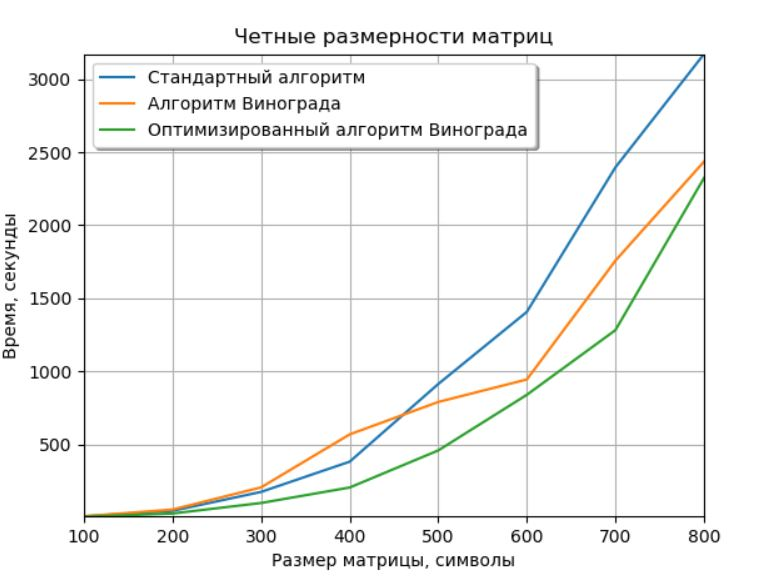
\includegraphics[width=0.8\linewidth, height = 0.5\textheight]{gr2}}
		\caption{Сравнение реализаций алгоритмов нахождения произведения матриц при четных размерностях.\centering}
		\label{image1}
	\end{figure}

	\begin{figure}[h]
	\center{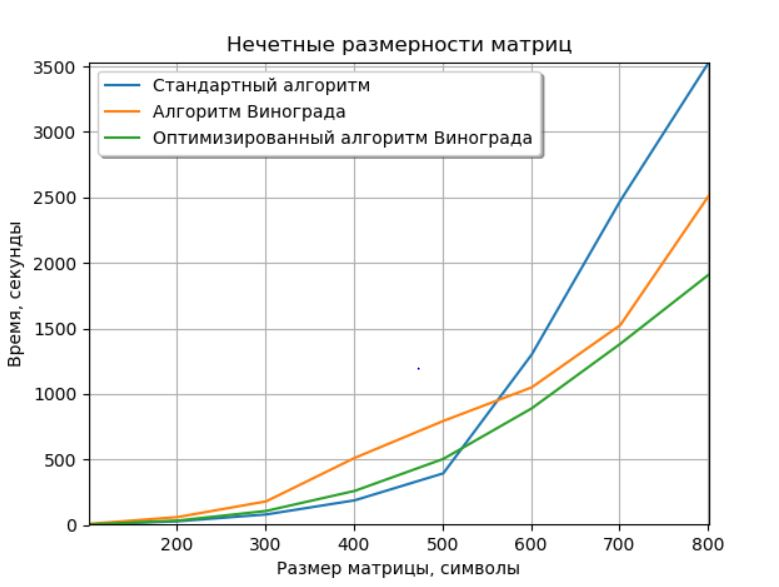
\includegraphics[width=0.8\linewidth, height = 0.5\textheight]{gr1}}
	\caption{Сравнение реализаций алгоритмов нахождения произведения матриц при нечетных размерностях.\centering}
	\label{image2}
	\end{figure}
	\clearpage
	
	
	\subsection{Вывод}
	В результате проведенных экспериментов были получены следующие выводы:
	\begin{enumerate}
		\item оптимизированный алгритм Винограда работает быстрее классического алгоритма;
		\item оптимизированный алгорити Винограда работает быстрее обычного алгоритма Винограда;
		\item по результатам тестирования на матрицах с нечётными размерностями видно, что неоптимизированный алгоритм Винограда работает медленнее, чем при работе с чётными размерностями;
		
	\end{enumerate}
	\clearpage
	
	
	\section*{Заключение}
	В данной лабораторной работе были реализованы и проанализированы три алгоритма умножения матриц:
	\begin{itemize}
		\item стандартный алгоритм умножения матриц;
		\item алгоритм Винограда;
		\item оптимизированный алгоритм Винограда;
	\end{itemize}

	В данной лабораторной работе была достигнута цель и были выполнены следующие задачи:
	\begin{enumerate}
		\item были описаны формулы расчета для двух алгоритмов: стандартного и алгоритма Винограда;
		\item были реализованы стандартный алгоритм умножения матриц и алгоритм Винограда;
		\item был реализован оптимизированный алгоритм Винограда;
		\item посчитана теоретическая оценка сложности трех алгоритмов;
		\item проведены замеры процессорного времени работы реализаций трех алгоритмов при четных и нечетных размерностях;
		
	\end{enumerate}
	\clearpage
	
	\begin{thebibliography}{5}
		\bibitem{what_is_python}	 
		Python:что нужно знать. [ЭЛ. РЕСУРС]\\
		Режим доступа: https://skillbox.ru/media/code/story\_buzunov/ \\
		(Дата обращения: 30.10.2020)
		
		\bibitem{timeit}
		Timeit в Python с примерами. [ЭЛ. РЕСУРС]\\
		Режим доступа: http://espressocode.top/timeit-python-examples/ \\
		(Дата обращения: 30.10.2020)
		\bibitem {standart}
		Умножение матриц. [ЭЛ. РЕСУРС] \\
		Режим доступа: http://algolib.narod.ru/Math/Matrix.html \\
		(Дата обращения: 30.10.20)\\
		
		\bibitem {difficulty}
		Знай сложности алгоритмов. [ЭЛ. РЕСУРС] \\
		Режим доступа: https://habr.com/ru/post/188010/ \\
		(Дата обращения: 30.10.20)\\
		
		\bibitem {intuit}
		Параллельные методы матричного умножения. [ЭЛ.РЕСУРС] \\
		Режим доступа: https://intuit.ru/studies/courses/2065/190/lecture/4954 \\
		(Дата обращения: 30.10.20)\\
	\end{thebibliography}




\end{document}
